% This file was created by matplotlib2tikz v0.6.15.
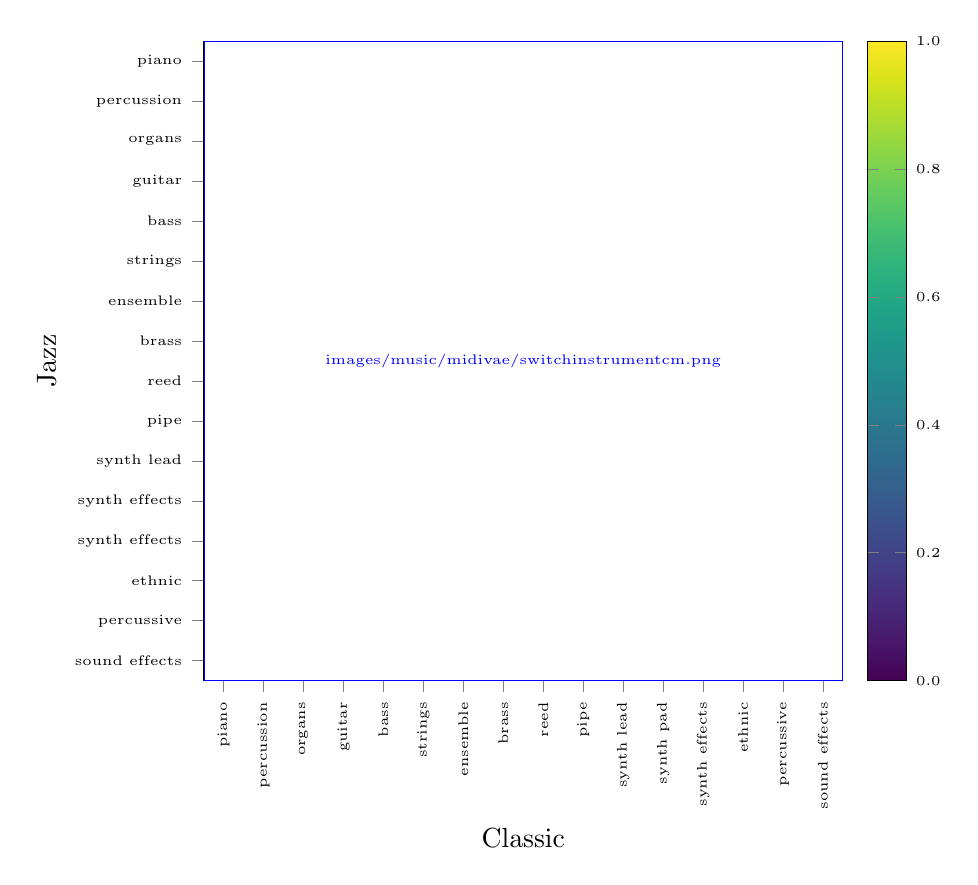
\begin{tikzpicture}

\begin{axis}[
% title={jazz switched to classic: Switched instruments:  51.34 percent},
xlabel={Classic},
ylabel={Jazz},
xmin=-0.5, xmax=15.5,
ymin=-0.5, ymax=15.5,
width=0.8\columnwidth,
height=0.8\columnwidth,
xtick={0,1,2,3,4,5,6,7,8,9,10,11,12,13,14,15},
xticklabels={piano,percussion,organs,guitar,bass,strings,ensemble,brass,reed,pipe,synth lead,synth pad,synth effects,ethnic,percussive,sound effects},
ytick={0,1,2,3,4,5,6,7,8,9,10,11,12,13,14,15},
% yticklabels={piano,percussion,organs,guitar,bass,strings,ensemble,brass,reed,pipe,synth lead,synth pad,synth effects,ethnic,percussive,sound effects},
yticklabels={sound effects,percussive,ethnic,synth effects,synth effects,synth lead,pipe,reed,brass,ensemble,strings,bass,guitar,organs,percussion,piano},
tick align=outside,
yticklabel style = {font=\tiny},
xticklabel style = {rotate=90,font=\tiny},
tick pos=left,
x grid style={lightgray!92.02614379084967!black},
y grid style={lightgray!92.02614379084967!black},
colorbar,
colormap/viridis,
point meta min=0,
point meta max=1,
colorbar style={font=\tiny, ytick={0,0.2,0.4,0.6,0.8,1},yticklabels={0.0,0.2,0.4,0.6,0.8,1.0},ylabel={}}
]
\addplot graphics [includegraphics cmd=\pgfimage,xmin=-0.5, xmax=15.5, ymin=15.5, ymax=-0.5] {images/music/midivae/switchinstrumentcm.png};
%\path [draw=black, fill opacity=0] (axis cs:0,15.5)
%--(axis cs:0,-0.5);

%\path [draw=black, fill opacity=0] (axis cs:1,15.5)
%--(axis cs:1,-0.5);

%\path [draw=black, fill opacity=0] (axis cs:-0.5,0)
%--(axis cs:15.5,0);

%\path [draw=black, fill opacity=0] (axis cs:-0.5,1)
%--(axis cs:15.5,1);

\end{axis}

\end{tikzpicture}